\section{Isis\-Dlm\-Routines.h File Reference}
\label{IsisDlmRoutines_8h}\index{IsisDlmRoutines.h@{IsisDlmRoutines.h}}


This graph shows which files directly or indirectly include this file:\begin{figure}[H]
\begin{center}
\leavevmode
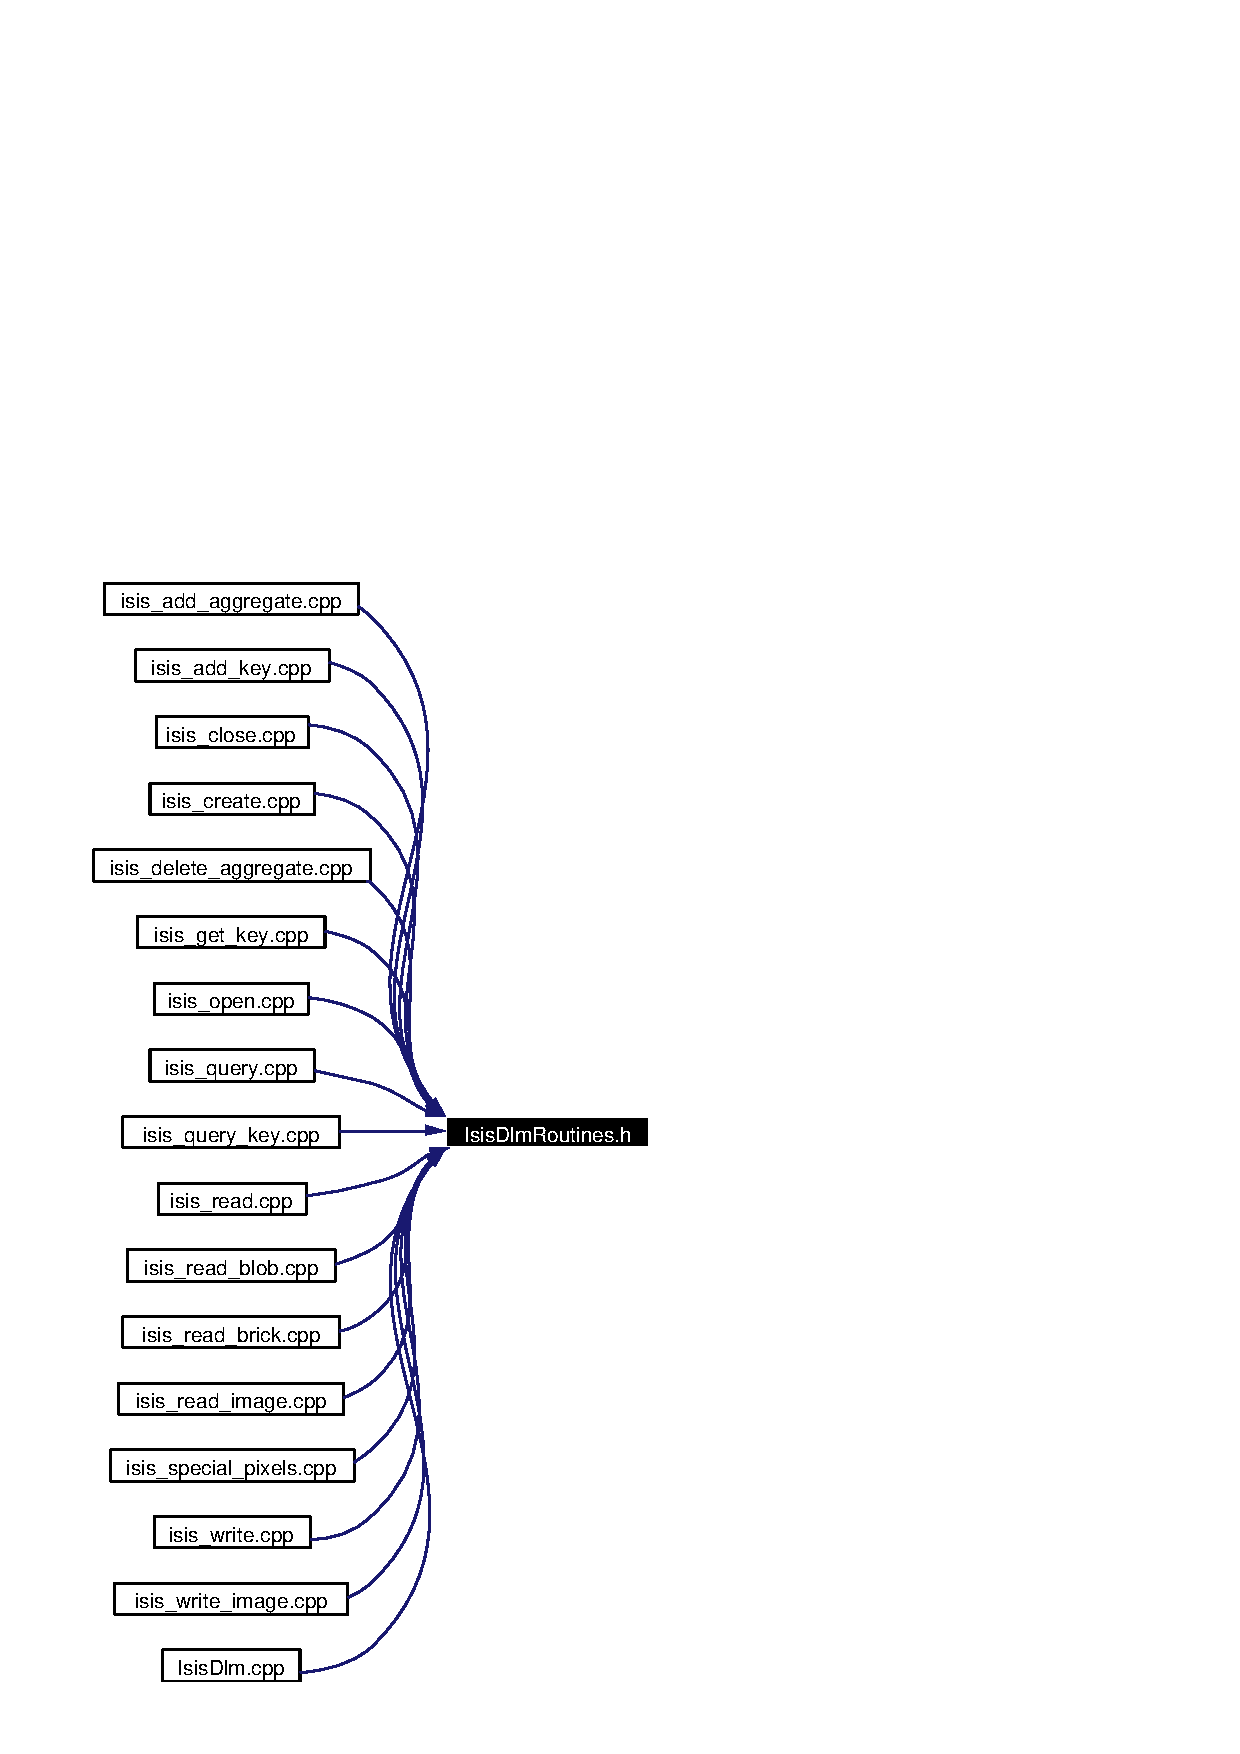
\includegraphics[width=160pt]{IsisDlmRoutines_8h__dep__incl}
\end{center}
\end{figure}
\subsection*{Namespaces}
\begin{CompactItemize}
\item 
namespace {\bf ISISDLM}
\end{CompactItemize}
\subsection*{Defines}
\begin{CompactItemize}
\item 
\#define {\bf Isis\-Dlm\-Routines\_\-h}
\end{CompactItemize}


\subsection{Define Documentation}
\index{IsisDlmRoutines.h@{Isis\-Dlm\-Routines.h}!IsisDlmRoutines_h@{IsisDlmRoutines\_\-h}}
\index{IsisDlmRoutines_h@{IsisDlmRoutines\_\-h}!IsisDlmRoutines.h@{Isis\-Dlm\-Routines.h}}
\subsubsection{\setlength{\rightskip}{0pt plus 5cm}\#define Isis\-Dlm\-Routines\_\-h}\label{IsisDlmRoutines_8h_a0}


Contains the declarations of all routines in this DLM This file will declare two routines for each DLM routine available in to the {\bf IDL} calling evironment.

The first routine is the initialization routine. This routine should declared using the Isis\-Dlm\-Init typedef. Here is an example of the declaration of the isis\_\-close\_\-init routine: 

\footnotesize\begin{verbatim}     extern int isis_close_init(IDL::IdlDlm &idl);
\end{verbatim}\normalsize


The second declaration is the {\bf IDL} DLM routine itself. This should use the Idl\-Rtn\-Def definition for its prototype: 

\footnotesize\begin{verbatim}     extern int isis_close(const IDL::IdlRtnDef &rtn, 
                           const IDL::IdlParameters &input, 
                           IDL::IdlParameters &output);
\end{verbatim}\normalsize


This allows for the implemention of the routine to be completely contained in a single implementation file.

\begin{Desc}
\item[Author:]Kris Becker, USGS, Flagstaff, Arizona \begin{Desc}
\item[Id]{\bf Isis\-Dlm\-Routines.h},v 1.2 2004/09/10 05:56:09 kbecker Exp \end{Desc}
\end{Desc}
